\documentclass{article}

\usepackage[main, final]{neurips_2026}
\usepackage[utf8]{inputenc}
\usepackage[T1]{fontenc}
\usepackage{hyperref}
\usepackage{url}
\usepackage{booktabs}
\usepackage{array}
\usepackage{amsfonts}
\usepackage{nicefrac}
\usepackage{microtype}
\usepackage{xcolor}
\usepackage{graphicx}
\usepackage{subcaption}
\usepackage{float}

\title{Efficient MPI Circle Rendering with Adaptive Heuristic Decomposition Methods}
\author{%
  An-Che Liang, Guan-Ming Chiu, Pei-Yu Wu\\
  National Taiwan University\\
  Team 12\\
}

\begin{document}

\maketitle

\section{Summary}
This project implements the required CRDR circle renderer in \texttt{renderer.c} and the optimized MPI implementation in \texttt{renderer\_mpi.c}. The final MPI renderer preserves the file-order semantics specified in \texttt{spec.pdf}: circles are stored back to front, so rendering records in input order ensures that later circles overwrite earlier circles exactly.

All benchmarked outputs were byte-identical to the provided golden PNG files. The benchmark data used in this report were generated with the commands \path{REPS=10 NPROCS="1 4 8 16 64" ./bench.sh} and \path{poetry run python scripts/generate_report_assets.py}.

The generated data and figures are stored in \path{data/testcase_metadata.csv}, \path{data/benchmark_results.csv}, \path{data/summary_16proc.csv}, \path{data/summary_64proc.csv}, \path{figure/strong_scaling_runtime.png}, \path{figure/speedup.png}, \path{figure/efficiency.png}, \path{figure/imbalance.png}, and \path{figure/problem_size_per_process.png}.

\section{Environment}
The experiments were conducted on Ubuntu 24.04.1 LTS running Linux kernel 6.8.0-100-generic. The host system used an Intel Xeon Platinum 8352V processor at 2.10 GHz with a topology of 2 sockets, 36 cores per socket, 2 threads per core, and 2 NUMA nodes. The MPI runtime was Open MPI 4.1.6, and the compiler was \texttt{mpicc} backed by GCC 13.3.0.

\begin{table}[H]
\centering
\caption{Experimental configuration used for benchmarking.}
\label{tab:environment}
\resizebox{\linewidth}{!}{%
\begin{tabular}{ll}
\toprule
Setting & Value \\
\midrule
Build command & \texttt{mpicc renderer\_mpi.c -o renderer\_mpi -lm -march=native} \\
Process counts & 1, 4, 8, 16, 64 \\
Single-node limit & Up to 16 MPI processes \\
64-process configuration & 4 nodes with 16 processes per node via \texttt{hosts} \\
Reported time & Median of 10 runs \\
Timing definition & Total wall time printed by \texttt{renderer\_mpi} \\
\bottomrule
\end{tabular}
}
\end{table}

\section{Implementation}
The final MPI renderer selects between two strategies at runtime according to the number of circles. Scenes with 500{,}000 circles or fewer use Mode A, named REPLICATE, whereas scenes above that threshold use Mode B, named PARTITION. The threshold was tuned empirically against benchmark data at 64 processes and can be overridden through the \texttt{RENDERER\_THRESHOLD} environment variable.

\subsection{Mode A: REPLICATE}
In Mode A, rank 0 reads the CRDR file and broadcasts all circle records to every rank. Each rank owns a cyclic stripe of image rows, where rank \(r\) owns rows \(r, r + P, r + 2P, \dots\), with \(P\) denoting the process count. Before rasterization, each rank prefilters the full record list to retain only circles whose bounding-box vertical range intersects its owned rows. The prefiltered list caches the bounding box and the first owned row, denoted \(y_{\mathrm{first}}\), so the inner raster loop remains branch-free with respect to ownership. Each rank rasterizes into a compact \(W \times \mathrm{local\_rows}\) RGB buffer, and \texttt{MPI\_Gatherv} collects the compact slices before rank 0 reinterleaves them into the final image.

Cyclic row ownership balances work even when circles cluster in a vertical region, which a contiguous block assignment cannot guarantee. The compact per-rank buffer also avoids allocating a full \(W \times H\) image on every process, which becomes increasingly important as \(P\) grows.

\subsection{Mode B: PARTITION}
In Mode B, rank 0 reads and broadcasts the full record array. A scatter-based distribution was measured to be approximately three times slower than broadcast on this cluster for equivalent payloads, so broadcast is used in both modes. Each rank then slices the record array locally: rank \(r\) owns a contiguous chunk of \(count/P\) consecutive records in file order, with rank 0 holding the earliest, back-most circles and rank \(P-1\) holding the latest, front-most circles. Each rank rasterizes its own records into a full \(W \times H\) buffer of \texttt{uint32\_t}-encoded pixels, where each pixel is packed as \( ((\mathrm{rank}+1) \ll 24) \;|\; R \ll 16 \;|\; G \ll 8 \;|\; B \). Untouched pixels remain zero. A collective \texttt{MPI\_Reduce} with \texttt{MPI\_MAX} across all ranks then selects the correct color per pixel, because a larger rank marker indicates that a later circle should win under the back-to-front painter semantics. Using the predefined \texttt{MPI\_MAX} operation on \texttt{MPI\_UINT32\_T} instead of a custom non-commutative \texttt{MPI\_Op} keeps the reduction on the hardware-accelerated collective path.

This mode reduces the per-rank rasterization cost to approximately \(1/P\) of the serial work, at the cost of a full-image \(W \times H \times 4\)-byte buffer on each rank and a reduction across all pixels.

\subsection{Common optimizations}
The implementation applies per-row analytic \(x\)-range trimming with \texttt{sqrtf}, followed by the exact circle-inside test, to avoid iterating over pixels that are clearly outside the circle. The renderer writes opaque RGB values directly, which matches the assignment format in which records contain only \texttt{uint8\_t} red, green, and blue components. The source also uses \texttt{\#pragma GCC optimize("O3", "unroll-loops")} because the official compile command does not specify an explicit optimization flag.

\section{Test Cases}
The binary metadata in \texttt{data/testcase\_metadata.csv} shows that the large cases use a 640\,$\times$\,480 image with 1M, 2M, and 4M circles. The special \texttt{imbalance\_c100000} case is smaller, using a 320\,$\times$\,240 image with 100K circles, but it has much larger radius variation. Its maximum radius is approximately 1998 pixels, compared with roughly 20 pixels for the regular large cases. This makes the case suitable for stressing load balance.

\begin{table}[t]
\centering
\caption{Summary of benchmark test cases.}
\label{tab:testcases}
\resizebox{\linewidth}{!}{%
\begin{tabular}{lrrrr}
\toprule
Testcase & Circles & Image & Mean radius & Max radius \\
\midrule
\texttt{imbalance\_c100000} & 100{,}000 & 320\,$\times$\,240 & 25.62 & 1998.10 \\
\texttt{medium\_c200000} & 200{,}000 & 640\,$\times$\,480 & 10.49 & 20.00 \\
\texttt{large\_c1000000} & 1{,}000{,}000 & 640\,$\times$\,480 & 10.50 & 20.00 \\
\texttt{large\_c2000000} & 2{,}000{,}000 & 640\,$\times$\,480 & 10.50 & 20.00 \\
\texttt{large\_c4000000} & 4{,}000{,}000 & 640\,$\times$\,480 & 10.50 & 20.00 \\
\bottomrule
\end{tabular}
}
\end{table}

\section{Benchmark Results}
The benchmark uses the median wall time across 10 repetitions for each testcase and process-count pair. The one-process MPI run serves as the serial baseline for speedup and efficiency because it exercises the same optimized renderer with \(P=1\).

\begin{figure}[t]
\centering
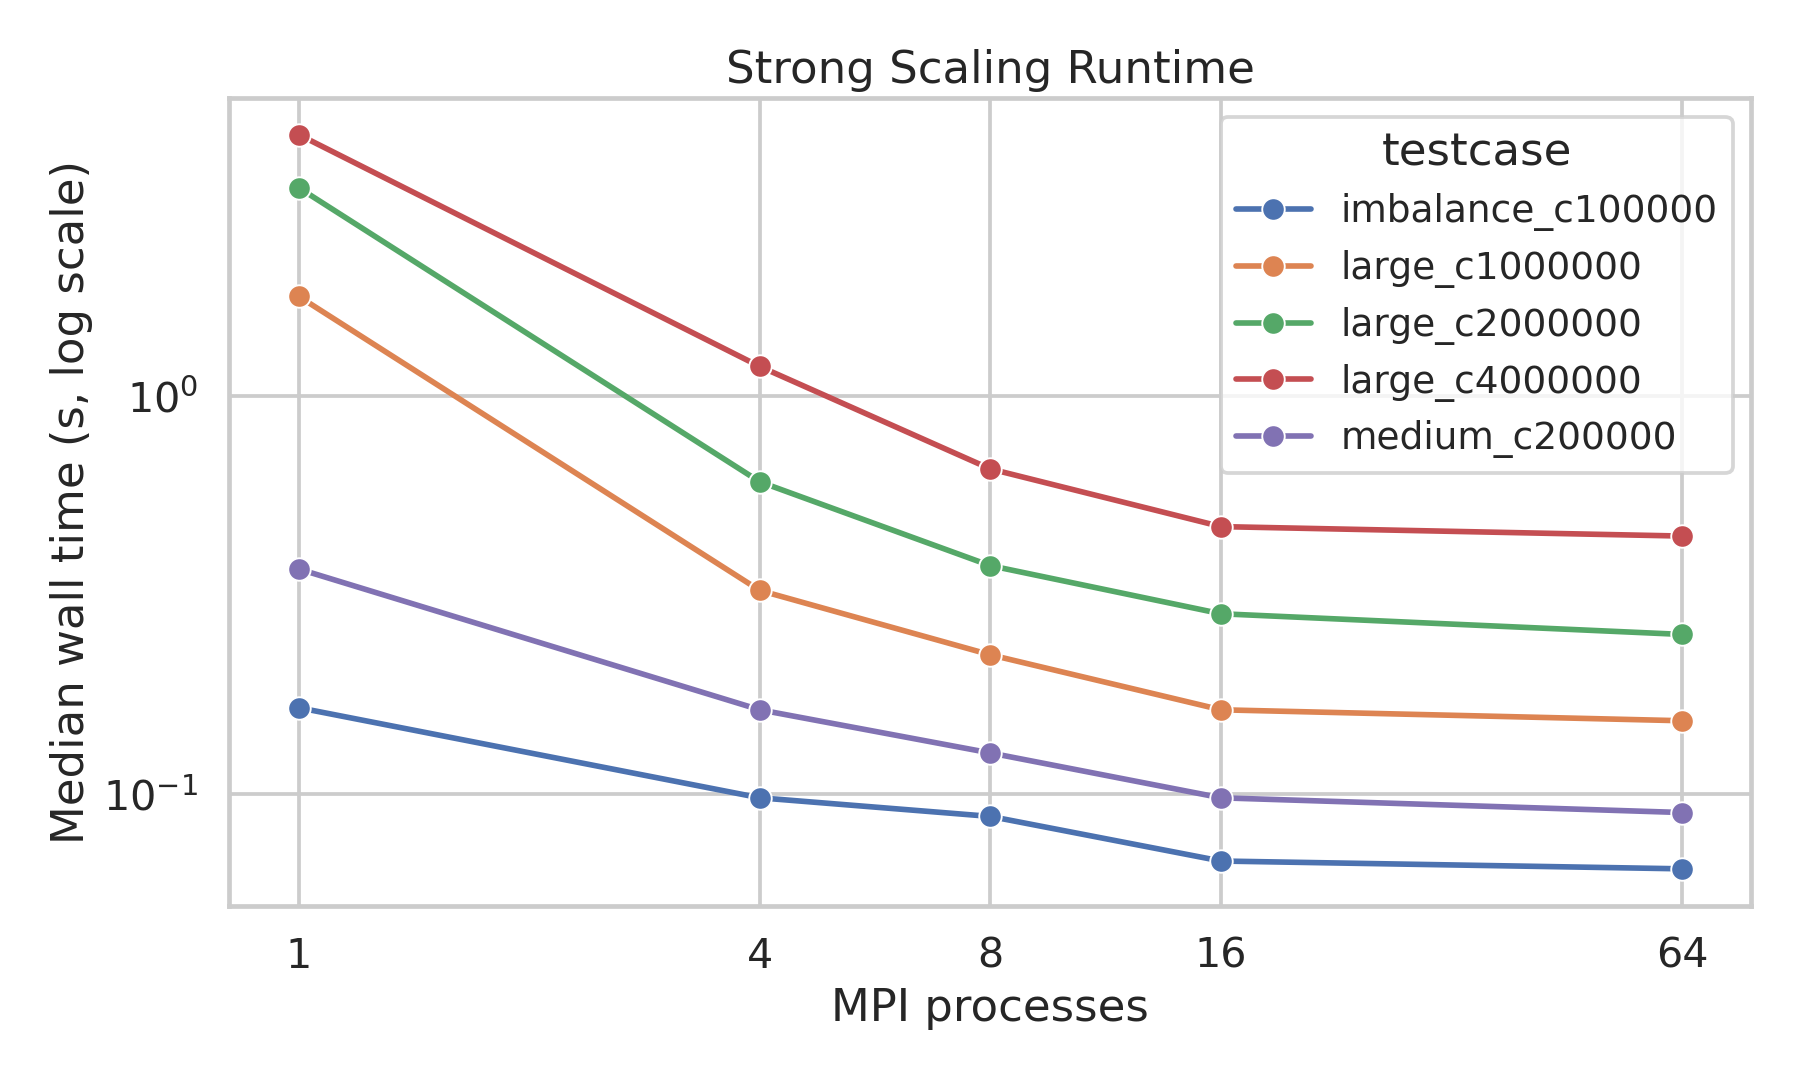
\includegraphics[width=0.9\linewidth]{figure/strong_scaling_runtime.png}
\caption{Strong-scaling runtime across process counts.}
\label{fig:runtime}
\end{figure}

\begin{figure}[t]
\centering
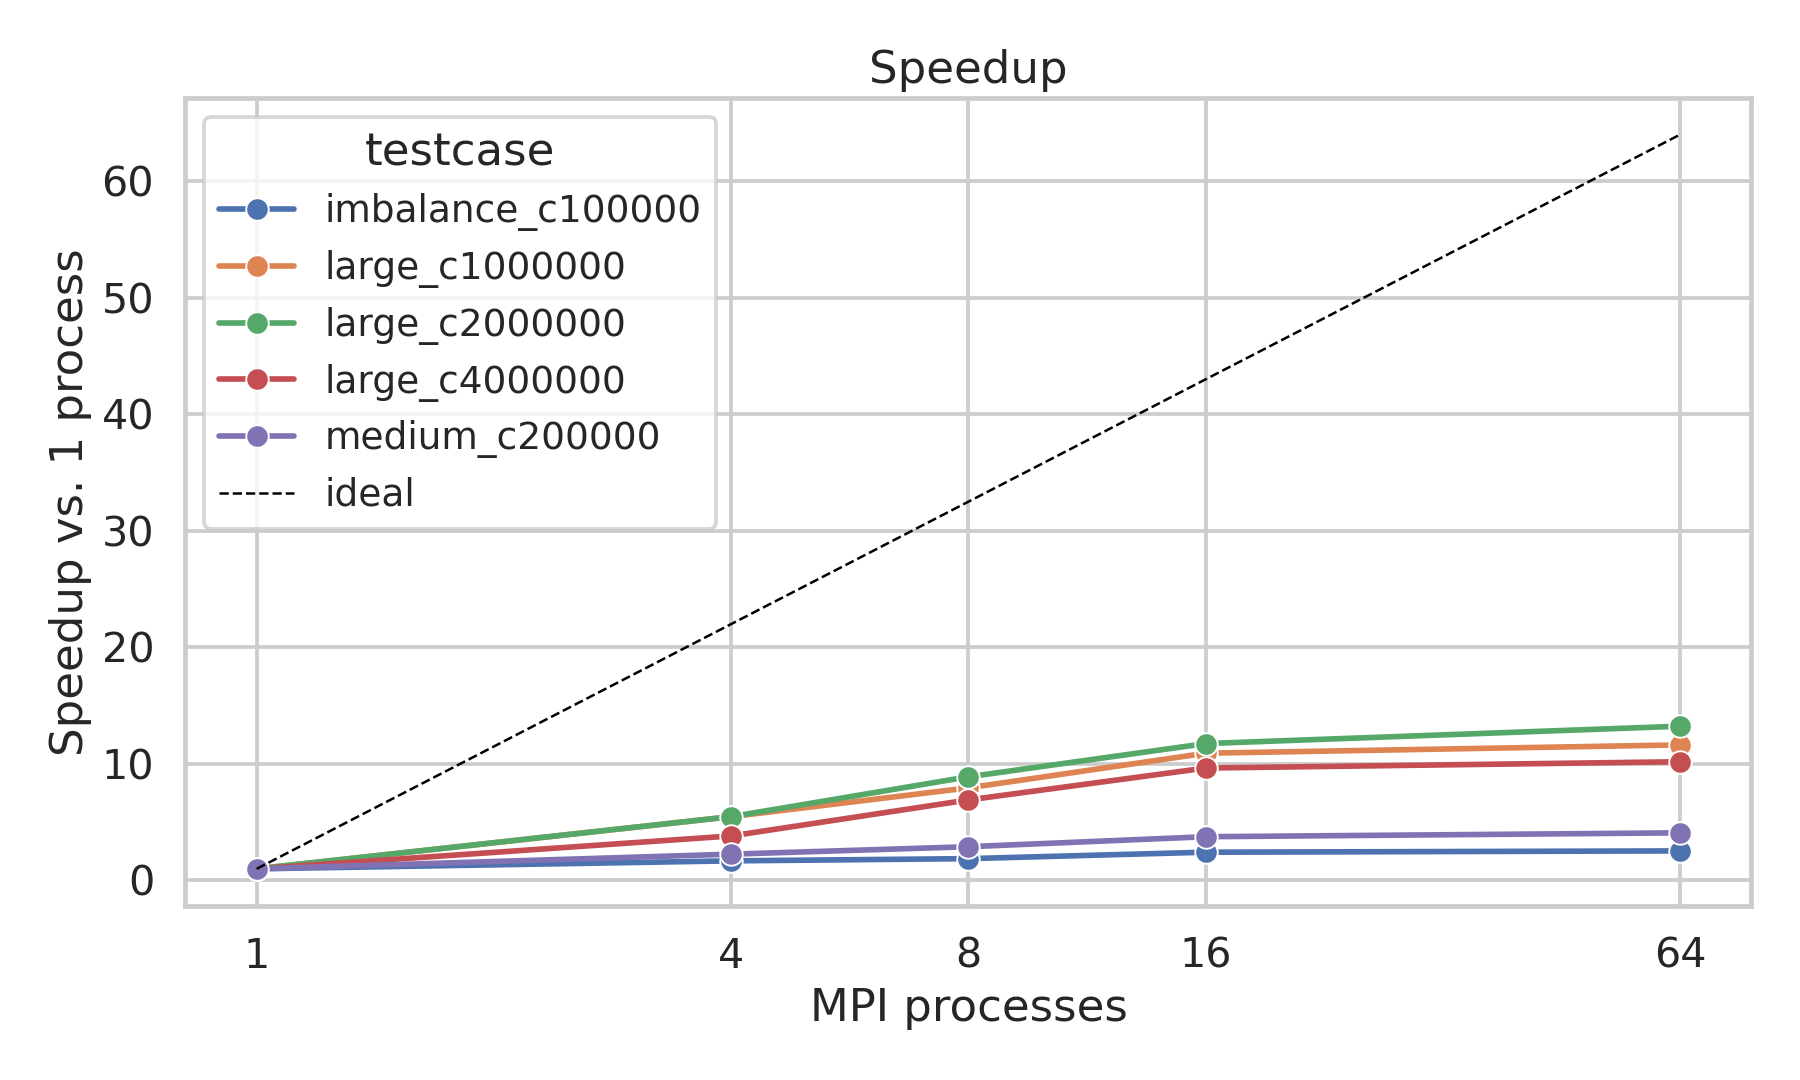
\includegraphics[width=0.9\linewidth]{figure/speedup.png}
\caption{Speedup across process counts.}
\label{fig:speedup}
\end{figure}

\begin{table}[t]
\centering
\caption{Median runtime, speedup, and efficiency for each testcase.}
\label{tab:benchmarks}
\resizebox{\linewidth}{!}{%
\begin{tabular}{lrrrrrrr}
\toprule
Testcase & 1 proc (s) & 4 proc (s) & 8 proc (s) & 16 proc (s) & 64 proc (s) & 64-proc speedup & 64-proc efficiency \\
\midrule
\texttt{imbalance\_c100000} & 0.165 & 0.098 & 0.088 & 0.068 & 0.065 & 2.54$\times$ & 4.0\% \\
\texttt{medium\_c200000} & 0.368 & 0.163 & 0.127 & 0.098 & 0.090 & 4.09$\times$ & 6.4\% \\
\texttt{large\_c1000000} & 1.780 & 0.325 & 0.224 & 0.163 & 0.153 & 11.63$\times$ & 18.2\% \\
\texttt{large\_c2000000} & 3.336 & 0.609 & 0.375 & 0.284 & 0.252 & 13.24$\times$ & 20.7\% \\
\texttt{large\_c4000000} & 4.534 & 1.186 & 0.656 & 0.470 & 0.445 & 10.19$\times$ & 15.9\% \\
\bottomrule
\end{tabular}
}
\end{table}

The best 64-process strong-scaling result is \texttt{large\_c2000000}, which improves from 3.336 s on one process to 0.252 s on 64 processes, corresponding to a 13.24\(\times\) speedup. On a single local node, the same case improves to 0.284 s on 16 processes, which is an 11.75\(\times\) speedup with 73.4\% efficiency. The smaller cases still improve, but their efficiency declines because fixed costs such as record broadcast, gather, PNG writing, MPI launch overhead, and multi-node communication occupy a larger share of total runtime.

\begin{figure}[t]
\centering
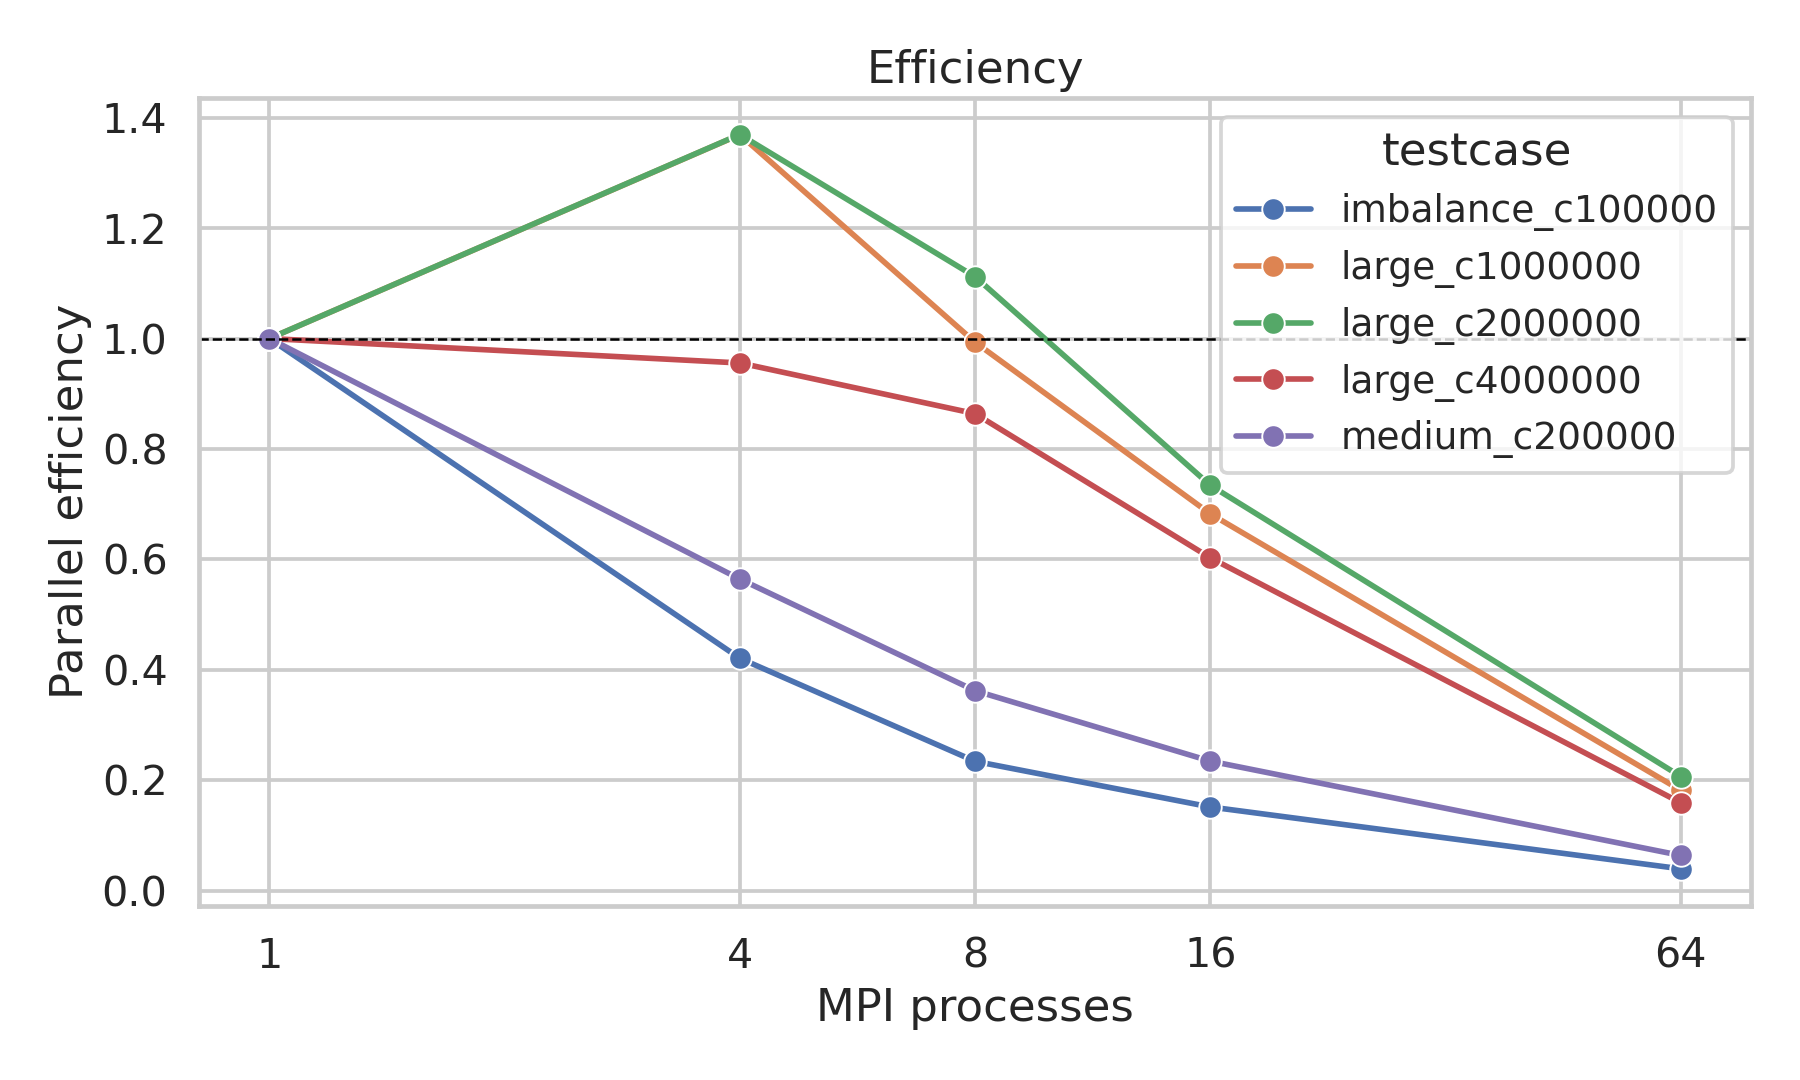
\includegraphics[width=0.9\linewidth]{figure/efficiency.png}
\caption{Parallel efficiency across process counts.}
\label{fig:efficiency}
\end{figure}

\section{Problem Size Per Process}
At 64 processes, throughput increases with larger scenes: 1.54 million circles per second for \texttt{imbalance\_c100000}, 2.22 million circles per second for \texttt{medium\_c200000}, 6.54 million circles per second for \texttt{large\_c1000000}, 7.94 million circles per second for \texttt{large\_c2000000}, and 8.99 million circles per second for \texttt{large\_c4000000}. These values are reflected in \texttt{data/summary\_64proc.csv} and \texttt{figure/problem\_size\_per\_process.png}.

\begin{figure}[t]
\centering
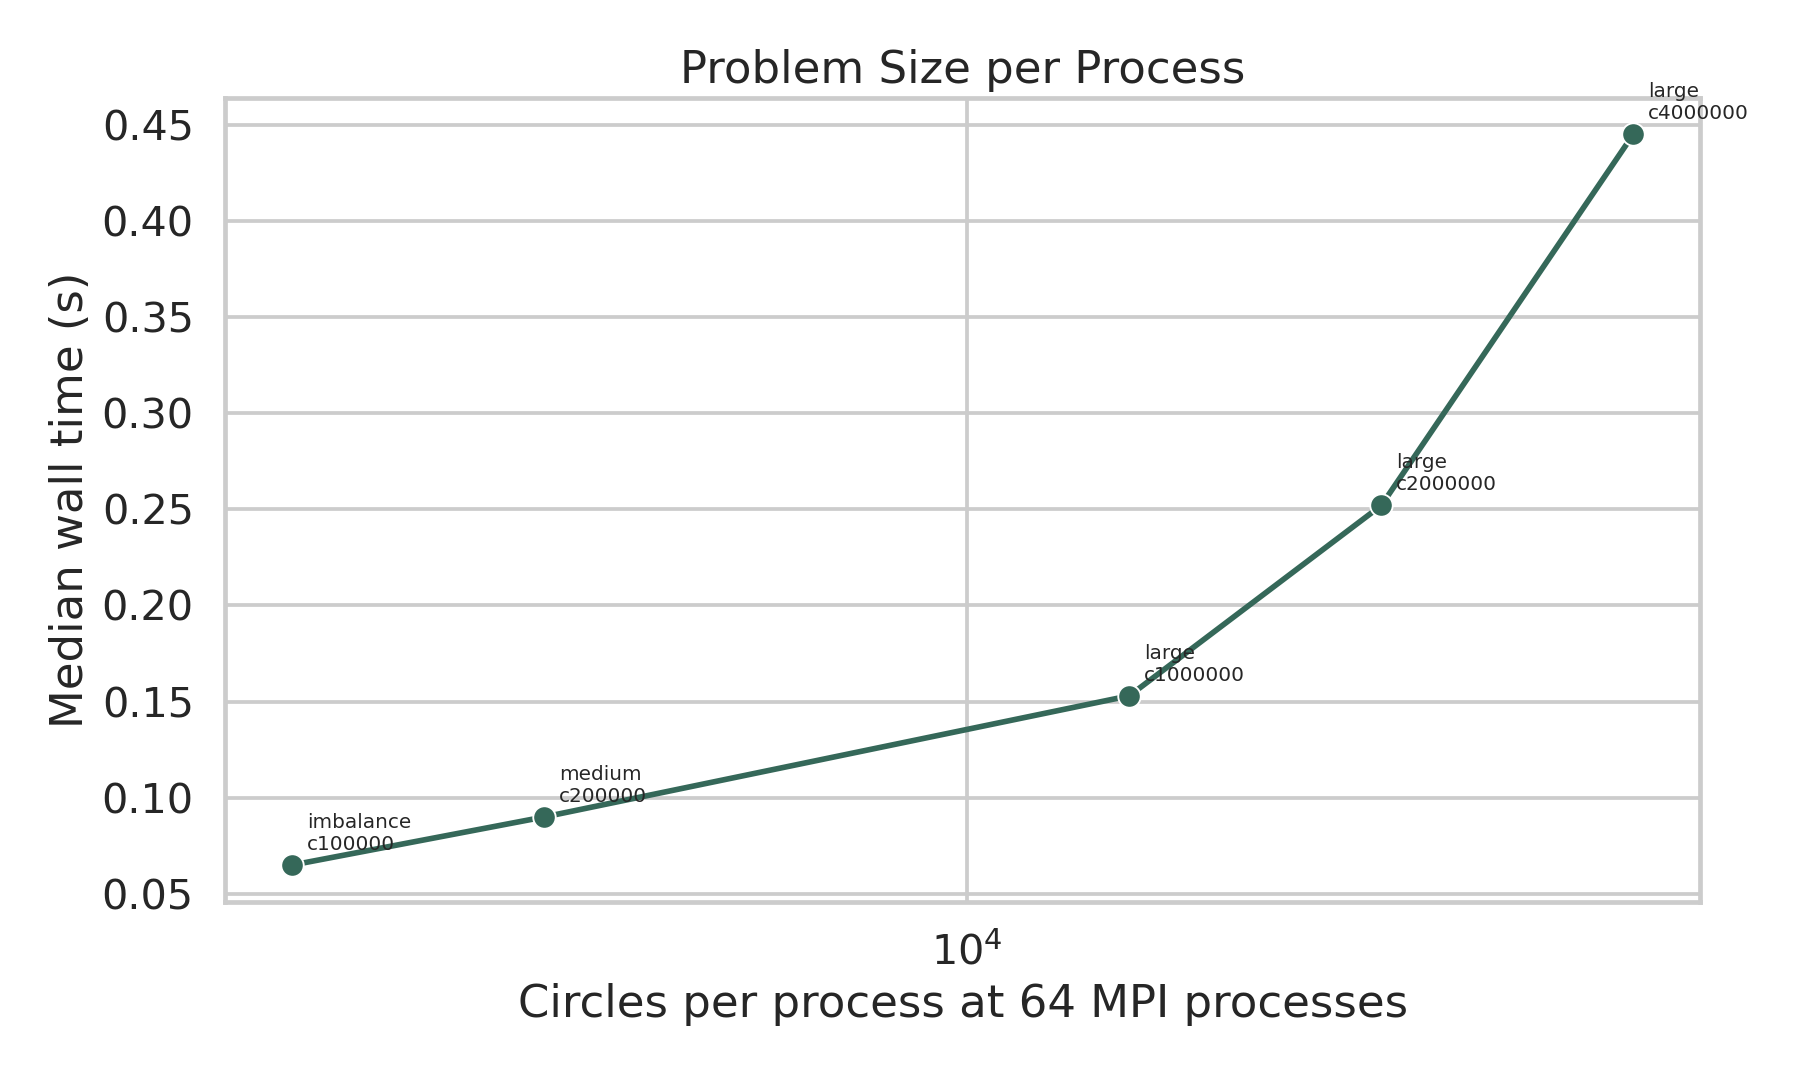
\includegraphics[width=0.9\linewidth]{figure/problem_size_per_process.png}
\caption{Throughput as a function of problem size at 64 processes.}
\label{fig:problem-size}
\end{figure}

The weak-scaling conclusion is mixed. More circles per process amortize fixed MPI and output costs, so throughput improves as the problem grows. However, wall time still increases from 0.153 s at 1M circles to 0.445 s at 4M circles on 64 processes because each process still loops over every circle and skips only the pixels outside its owned rows. The algorithm scales well for strong scaling, but it is not true weak scaling because both broadcast size and per-rank circle iteration grow with total circle count.

\section{Load Balance}
The renderer logs per-rank render time statistics and reports imbalance as \(\max / \mathrm{mean}\). The measured imbalance values are recorded in \texttt{data/benchmark\_results.csv} and plotted in \texttt{figure/imbalance.png}.

\begin{figure}[t]
\centering
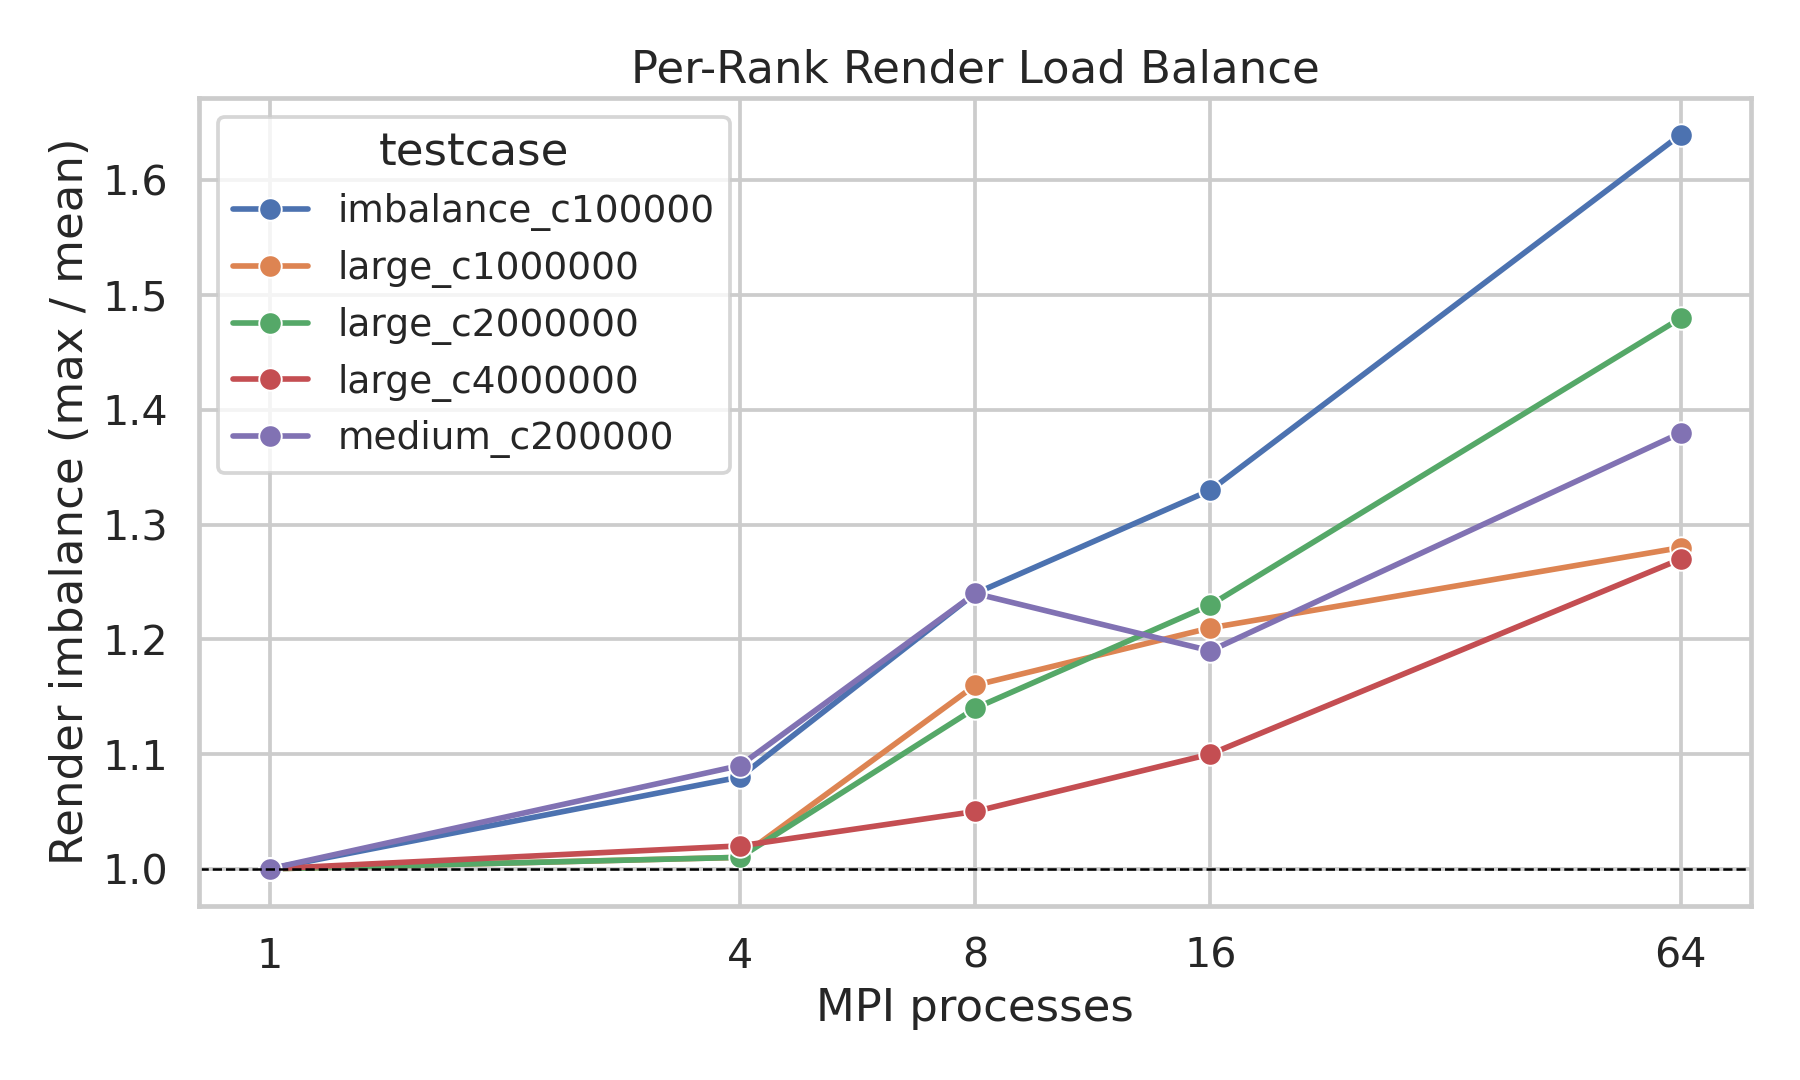
\includegraphics[width=0.9\linewidth]{figure/imbalance.png}
\caption{Per-rank render imbalance across benchmark cases.}
\label{fig:imbalance}
\end{figure}

The three large scenes, namely \texttt{large\_c1000000}, \texttt{large\_c2000000}, and \texttt{large\_c4000000}, use Mode B. In this mode each rank renders a disjoint slice of records into a full image, so imbalance reflects variation in circle counts across ranks. Because records are split evenly, imbalance arises from radius variation rather than spatial clustering. At 16 processes the imbalance is 1.21, 1.23, and 1.10 respectively, and at 64 processes it is 1.28, 1.48, and 1.27. These values remain controlled because the large scenes use uniformly sized circles with a maximum radius of 20 pixels.

The two smaller scenes, \texttt{imbalance\_c100000} and \texttt{medium\_c200000}, use Mode A. In this mode each rank rasterizes prefiltered circles into its cyclic row stripe, so imbalance reflects whether very large circles disproportionately cover certain rows. At 64 processes, \texttt{medium\_c200000} has imbalance 1.38, and \texttt{imbalance\_c100000} has the highest imbalance at 1.64. The special imbalance case contains circles with radii up to 1998 pixels in a 320\,$\times$\,240 image, so a single circle can span almost the full image height. Cyclic row distribution spreads that coverage across all ranks rather than concentrating it in one contiguous block, which keeps imbalance below 2\(\times\) despite the extreme radius variation. Even with this imbalance, wall time improves from 0.165 s on one process to 0.065 s on 64 processes.

\section{Conclusion}
The MPI renderer is correct on all benchmarked test cases and demonstrates meaningful strong scaling under the 64-process competition configuration. The adaptive strategy, which switches from cyclic row decomposition in Mode A for smaller scene sizes to record partitioning with a painter reduction in Mode B for larger scene sizes, provides good performance across both regimes. The best measured result is a 13.24\(\times\) speedup on \path{large_c2000000} under Mode B, while the 4M-circle case achieves the highest throughput at 8.99 million circles per second.

The main cost in Mode A is that every rank scans all records during prefiltering, so broadcast size and prefilter time grow with total circle count regardless of \(P\). Mode B addresses this by giving each rank only \(count/P\) records to rasterize, but it trades that improvement for a full-image \texttt{uint32\_t} buffer per rank and a pixel-level \texttt{MPI\_MAX} reduction. The threshold of 500,000 circles was chosen where the reduction overhead in Mode B becomes cheaper than the per-rank prefilter scan cost in Mode A at 64 processes.

\end{document}
